% Provenance (never printed): see sources/outline_sources.md (Year 2: natural hazards and risks
% quantified --- recurrence, probabilistic hazard, slope stability, tsunamis, floods, warning).
% Terminology from the UN report A/71/644 (UNDRR); the 475-year convention from the USGS
% Earthquake Hazards 201 page; the ground-motion prediction equation of Boore, Joyner and Fumal
% (USGS Open-File Report 93-509); run-ups from the NOAA NCEI tsunami database; the 1999 Vargas
% debris flows from USGS Open-File Report 01-0144. Ledger rows in sources/ledger/book4.md;
% curves and numbers from figdata/bachelor-2/hazards.py and the Book 4 second-writer scratch
% calculator calc/ch28.py. Hazards are described and quantified physically only: no advice.
\chapter{भूवैज्ञानिक संकट और जोखिम}\label{ch:b2:geological-hazards}

जिस भू-गति का अतिक्रमण औसतन 475 वर्षों में एक बार होता है, उसके लिए अभिकल्पित किसी भवन के अपने पचास-वर्षीय
जीवनकाल में उससे सामना होने की संभावना दस में एक है। दोनों कथन एक ही संख्या हैं, जिसे दो तरह से
पढ़ा गया है, और उनके बीच आना-जाना संकट-विज्ञान का दैनिक काम है। यह अध्याय
उसके उपकरण बनाता है: दुर्लभ घटनाओं की प्रायिकता, किसी स्थल का \omterm{def:b2:geological-hazards:psha}{संकट वक्र}, किसी ढाल का
स्थायित्व, सुनामी का वेग और आरोहण, बाढ़ों की आवृत्ति, और वह भौतिकी जो तय करती है कि
हर संकट कितनी चेतावनी दे सकता है।
% ledger: usgs:eh201-475

\begin{recall}
\textbf{स्कूल की पुस्तकों से}: प्राकृतिक संकट, प्राकृतिक आपदा और भूस्खलन; सुभेद्यता,
जोखिम, रोकथाम और संकट मानचित्र; सुनामी; बाढ़ का \omterm{def:b2:geological-hazards:return}{पुनरावृत्ति काल}, और कोटि-सूत्र $T = (n + 1)/m$,
जो $n$ वार्षिक शिखरों के अभिलेख के लिए है। \textbf{पुस्तक 3 (स्नातक वर्ष 1) से}:
गुटेनबर्ग--रिक्टर नियम $\log_{10} N(\geq M) = a - bM$ और उसका b-मान; भूकंपीय आघूर्ण और आघूर्ण
परिमाण; छिद्र-द्रव दाब, प्रभावी प्रतिबल $\sigma' = \sigma - u$ और कूलॉम्ब विभंग
कसौटी $\tau = c' + \sigma' \tan\varphi'$। \textbf{\cref{ch:b2:eruptive-styles} से}: पायरोक्लास्टिक
घनत्व धाराएँ, \omterm{def:b2:eruptive-styles:lahar}{लाहार} और टेफ़्रा-पात। \textbf{गणित की पुस्तकों से}: प्वासों और
घातांकी बंटन, प्रसामान्य बंटन और उसका बंटन फलन $\Phi$।
\textbf{भौतिकी की पुस्तकों के स्नातक वर्ष 2 खंड से}: सतही गुरुत्व तरंगों का परिक्षेपण संबंध,
$\omega^2 = gk\tanh(kh)$।
\end{recall}

\section{संकट, उद्भासन और जोखिम}\label{sec:b2:geological-hazards:risk}

\begin{definition}[भूवैज्ञानिक संकट, उद्भासन, आपदा जोखिम]\label{def:b2:geological-hazards:risk}
\emph{भूवैज्ञानिक संकट}\index{भूवैज्ञानिक संकट} एक प्रक्रम या परिघटना है जो पृथ्वी के आंतरिक
प्रक्रमों से उत्पन्न होती है --- भूकंप, उद्गार, भूस्खलन या \omterm{def:b2:geological-hazards:slope}{मलबा-प्रवाह} जैसा कोई
द्रव्यमान-संचलन --- और जिससे जीवन की हानि, चोट, क्षति या व्यवधान हो सकता है। उसकी पहचान
उसके स्थान, उसकी तीव्रता या परिमाण, और उसकी आवृत्ति या प्रायिकता से होती है। किसी संकट के प्रति
\emph{उद्भासन}\index{उद्भासन (संकट के प्रति)} उन लोगों, भवनों, अवसंरचना और अन्य परिसंपत्तियों की
स्थिति है जो वहाँ स्थित हैं जहाँ तक संकट पहुँच सकता है, जिसे उनकी संख्या या उनके मूल्य से मापा जाता है।
\emph{आपदा जोखिम}\index{आपदा जोखिम} जीवन, स्वास्थ्य या परिसंपत्तियों की वह संभावित हानि है जो किसी
दी गई अवधि में हो सकती है, और जिसे संकट, उद्भासन और उद्भासित वस्तुओं की सुभेद्यता से
प्रायिकतात्मक रूप से निर्धारित किया जाता है।
\end{definition}
% ledger: undrr:hazard, undrr:geological, undrr:exposure, undrr:disaster-risk, undrr:vulnerability

अंतरराष्ट्रीय शब्दावली सुनामियों को अलग वर्ग में रखती है: भूकंपों और अन्य भूवैज्ञानिक घटनाओं से उत्पन्न होकर,
वे एक महासागरीय प्रक्रम बन जाती हैं और एक तटीय, जल-संबंधी संकट के रूप में प्रहार करती हैं।
यह अध्याय उन्हें दूसरों के साथ ही लेता है, क्योंकि उनका स्रोत भूवैज्ञानिक है।
% ledger: undrr:geological

परिभाषा में एक गुणनफल छिपा है। यदि तीव्रता $i$ की घटनाएँ एक वार्षिक दर
$\lambda_i$ से होती हैं, यदि उद्भासित परिसंपत्तियों का मूल्य $E$ है, और यदि तीव्रता $i$ की एक घटना उनका
एक अंश $V_i$ नष्ट करती है (सुभेद्यता, 0 और 1 के बीच), तो अपेक्षित वार्षिक हानि है
\begin{equation}
L = \sum_i \lambda_i \, E \, V_i ,
\label{eq:b2:geological-hazards:loss}
\end{equation}
जिसे प्रायः जोखिम = संकट $\times$ \omterm{def:b2:geological-hazards:risk}{उद्भासन} $\times$ सुभेद्यता के रूप में संक्षिप्त किया जाता है। जोखिम तब
लुप्त हो जाता है जब कोई भी गुणक लुप्त हो: किसी ख़ाली द्वीप पर एक प्रचंड ज्वालामुखी, किसी शांत \omterm{def:b2:precambrian-earth:craton}{क्रेटॉन} पर एक
भीड़-भरा नगर, या कंपन को सहने वाले भवन। संकट-विज्ञान पहला गुणक मापता है; नीचे का चित्र
उसे तीनों के बीच रखता है।

\begin{omfigure}
\centering
\begin{tikzpicture}[font=\small]
\fill[omThm!14] (90:1.05) circle (1.55);
\fill[omDef!14] (210:1.05) circle (1.55);
\fill[black!8] (330:1.05) circle (1.55);
\begin{scope}
\clip (90:1.05) circle (1.55);
\clip (210:1.05) circle (1.55);
\fill[omThm!45!omDef!45] (330:1.05) circle (1.55);
\end{scope}
\draw[omThm, thick] (90:1.05) circle (1.55);
\draw[omDef, thick] (210:1.05) circle (1.55);
\draw[black!60, thick] (330:1.05) circle (1.55);
\node[align=center, anchor=south] at (0,2.65) {\textbf{संकट} {\scriptsize (दर $\lambda_i$, तीव्रता)}};
\node[align=right, anchor=east] at (-2.55,-1.35) {\textbf{उद्भासन}\\[-1pt]{\scriptsize परिसंपत्तियाँ $E$}};
\node[align=left, anchor=west] at (2.55,-1.35) {\textbf{सुभेद्यता}\\[-1pt]{\scriptsize नष्ट अंश $V_i$}};
\node[align=center, font=\scriptsize\bfseries] at (0,0) {जोखिम};
\end{tikzpicture}
\par\smallskip{\small \omterm{def:b2:geological-hazards:risk}{आपदा जोखिम} के तीन गुणक। अपेक्षित हानि केवल वहीं शून्येतर है जहाँ
तीनों अतिव्यापित होते हैं: एक संकट जो किसी उद्भासित और क्षतिग्रस्त हो सकने वाली वस्तु तक पहुँचता है।}
\end{omfigure}

\section{दुर्लभ घटनाओं की प्रायिकता}\label{sec:b2:geological-hazards:probability}

\begin{definition}[पुनरावृत्ति काल]\label{def:b2:geological-hazards:return}
मान लीजिए किसी दिए गए प्रकार की घटनाएँ --- किसी विसर्जन से ऊपर की बाढ़, किसी स्तर से ऊपर की भू-गति,
किसी परिमाण से ऊपर का भूकंप --- एक माध्य वार्षिक दर $\lambda$ से होती हैं। उनका \emph{पुनरावृत्ति
काल}\index{पुनरावृत्ति काल} $T = 1/\lambda$ है: उनमें से दो के बीच का माध्य अंतराल, और उनकी वार्षिक
दर का व्युत्क्रम, कोई समय-सारणी नहीं।
\end{definition}
% ledger: usgs:eh201-475

\begin{definition}[अतिक्रमण प्रायिकता]\label{def:b2:geological-hazards:poisson}
किसी \omterm{def:b2:geological-hazards:risk}{उद्भासन} काल $t$ में किसी स्तर की \emph{अतिक्रमण प्रायिकता}\index{अतिक्रमण प्रायिकता}
वह प्रायिकता है कि $t$ के दौरान वह स्तर कम से कम एक बार बराबर किया जाए या पार किया जाए।
\end{definition}

\begin{proposition}[प्वासों पुनरावृत्ति मॉडल]\label{prop:b2:geological-hazards:poisson}
मान लीजिए घटनाएँ एक समय में एक\index{प्वासों पुनरावृत्ति मॉडल}, एक-दूसरे से और बीते समय से
स्वतंत्र रूप से, एक स्थिर माध्य दर $\lambda = 1/T$ से होती हैं। तब घटनाओं की संख्या $N$, समय $t$ में,
माध्य $\lambda t$ वाले प्वासों बंटन का अनुसरण करती है; $t$ में \omterm{def:b2:geological-hazards:poisson}{अतिक्रमण
प्रायिकता} है
\begin{equation}
P(t) = 1 - e^{-t/T};
\label{eq:b2:geological-hazards:poisson}
\end{equation}
और क्रमागत घटनाओं के बीच का अंतराल माध्य $T$ वाले घातांकी बंटन का अनुसरण करता है।
\end{proposition}

\begin{proof}
मान लीजिए $P_k(t)$ वह प्रायिकता है कि $k$ घटनाएँ $[0, t]$ में हों। एक लघु अंतराल $\mathrm{d}t$ में एक
घटना प्रायिकता $\lambda\,\mathrm{d}t$ के साथ होती है, अतीत से स्वतंत्र, और दो घटनाएँ उच्च कोटि की
प्रायिकता के साथ। अतः $P_0(t + \mathrm{d}t) = P_0(t)(1 - \lambda\,\mathrm{d}t)$, यानी
$P_0' = -\lambda P_0$, जहाँ $P_0(0) = 1$: $P_0(t) = e^{-\lambda t}$, और $P(t) = 1 - P_0(t)$। इसी
तरह $P_k' = \lambda(P_{k-1} - P_k)$, $k \geq 1$ के लिए, जिसे आगमन से हल किया जाता है:
$P_k(t) = (\lambda t)^k e^{-\lambda t}/k!$, माध्य $\lambda t$ वाला प्वासों बंटन। किसी घटना से
आरंभ करने पर, वही तर्क यह प्रायिकता देता है कि अगली घटना $t$ के बाद आए:
$e^{-\lambda t}$, घातांकी बंटन का उत्तरजीविता फलन, जिसका माध्य
$\int_0^\infty e^{-\lambda t}\,\mathrm{d}t = 1/\lambda = T$ है।
\end{proof}

दो परिणाम हर जगह प्रयुक्त होते हैं। प्रायिकता $p$ के लिए, \omterm{def:b2:geological-hazards:risk}{उद्भासन} काल $t$ में, \omterm{def:b2:geological-hazards:return}{पुनरावृत्ति
काल} $T = -t/\ln(1 - p)$ है: 50 वर्षों में \qty{10}{\percent} से $T = 50/0.10536 =
474.6$ वर्ष मिलता है, भवन-संहिताओं की ``475-वर्षीय'' गति, और 50 वर्षों में \qty{2}{\percent}
से 2475 वर्ष। और जब $t \ll T$, तो $P \approx t/T$: दर को प्रति वर्ष एक
प्रायिकता के रूप में पढ़ा जा सकता है। इसके विपरीत, एक पूरे \omterm{def:b2:geological-hazards:return}{पुनरावृत्ति काल} पर प्रायिकता $1 - e^{-1} =
\qty{63}{\percent}$ है, 1 नहीं। नीचे का चित्र (बाएँ) तीन \omterm{def:b2:geological-hazards:return}{पुनरावृत्ति कालों} के लिए
\eqref{eq:b2:geological-hazards:poisson} खींचता है।
% ledger: usgs:eh201-475
% values: T 474.561 and 2474.92 years; P(50|475) 0.0999 (hazards.py numbers)

क्या मॉडल सत्य है? कम से कम 7 परिमाण के भूकंपों की वैश्विक सूची में 1976 से 2025 तक 696 घटनाएँ हैं,
695 अंतराल, जिनका माध्य 26.2 दिन है। यदि वे एक प्वासों प्रक्रम होते, तो
$t$ से लंबे अंतरालों का अंश $e^{-t/26.2}$ होता, लघुगणकीय अक्ष पर एक सीधी रेखा।
नीचे का चित्र (दाएँ) दिखाता है कि वह लगभग वैसा ही है: \qty{30.4}{\percent} अंतराल
30 दिनों से लंबे हैं, मॉडल के \qty{31.8}{\percent} के सामने, और अंतरालों का मानक विचलन
उनके माध्य का 1.07 गुना है, ठीक 1 के सामने। दोष लघु अंतरालों पर है: 36 जोड़े
एक ही दिन पड़ते हैं, पश्चकंप और युग्म-भूकंप जिन्हें एक स्मृतिहीन प्रक्रम गुच्छित नहीं करता। इसलिए संकट
मानचित्र किसी सूची से आश्रित घटनाओं को हटा देते हैं, यानी उसका विगुच्छन करते हैं, ताकि
शेष मुख्य भूकंपों को एक प्वासों प्रक्रम माना जा सके; परिमाण के अनुसार उनकी दरें
गुटेनबर्ग--रिक्टर नियम से आती हैं।
% ledger: data:usgs-comcat, usgs:eh201-poisson
% values: m7_events 696, mean 26.2245 d, cv 1.06891, same-day 36, frac>30 d 0.303597 vs 0.318552

\begin{omfigure}
\centering
\begin{minipage}[b]{0.49\linewidth}\centering
\begin{tikzpicture}
\begin{axis}[omrecord, width=0.96\linewidth, height=5.2cm, xmin=0, xmax=200, ymin=0, ymax=1,
  xlabel={उद्भासन काल $t$ (वर्ष)}, ylabel={अतिक्रमण प्रायिकता},
  tick label style={font=\scriptsize}, label style={font=\small},
  xtick={0,50,100,150,200}, ytick={0,0.2,...,1}]
% computed in figdata/bachelor-2/hazards.py part poisson
\addplot[omThm, line width=1pt] table[x=t_yr, y=P50] {figdata/out/bachelor-2-hazards-poisson.dat};
\addplot[omDef, line width=1pt] table[x=t_yr, y=P475] {figdata/out/bachelor-2-hazards-poisson.dat};
\addplot[black!70, line width=1pt, densely dashed] table[x=t_yr, y=P2475] {figdata/out/bachelor-2-hazards-poisson.dat};
\draw[black!50, densely dotted] (axis cs:50,0) -- (axis cs:50,1);
\fill[omDef] (axis cs:50,0.1) circle (1.8pt);
\node[font=\scriptsize, text=omThm, anchor=west] at (axis cs:62,0.86) {$T = 50$};
\node[font=\scriptsize, text=omDef, anchor=west] at (axis cs:120,0.34) {$T = 475$};
\node[font=\scriptsize, text=black!70, anchor=west] at (axis cs:120,0.12) {$T = 2475$};
\node[font=\scriptsize, anchor=west, text=omDef] at (axis cs:52,0.2) {\qty{10}{\percent}};
\end{axis}
\end{tikzpicture}
\end{minipage}\hfill
\begin{minipage}[b]{0.49\linewidth}\centering
\begin{tikzpicture}
\begin{axis}[omrecord, width=0.93\linewidth, height=5.2cm, xmin=0, xmax=120, ymode=log,
  ymin=0.008, ymax=1.1, xlabel={अंतराल $t$ (दिन)}, ylabel={$> t$ अंतरालों का अंश},
  tick label style={font=\scriptsize}, label style={font=\small}, xtick={0,30,60,90,120},
  legend style={at={(0.03,0.03)}, anchor=south west, font=\scriptsize, draw=black!30},
  legend cell align=left]
% computed in figdata/bachelor-2/hazards.py part survival; ledger: data:usgs-comcat
\addplot[omThm, only marks, mark=*, mark size=1.2pt] table[x=t_day, y=observed] {figdata/out/bachelor-2-hazards-survival.dat};
\addlegendentry{$M \geq 7$, 1976--2025}
\addplot[black, line width=0.9pt] table[x=t_day, y=poisson] {figdata/out/bachelor-2-hazards-survival.dat};
\addlegendentry{प्वासों, माध्य 26.2 दिन}
\end{axis}
\end{tikzpicture}
\end{minipage}
\par\smallskip{\small बाएँ: 50, 475 और 2475 वर्षों के \omterm{def:b2:geological-hazards:return}{पुनरावृत्ति कालों} के लिए \omterm{def:b2:geological-hazards:risk}{उद्भासन} काल $t$ में
कम से कम एक घटना की प्रायिकता; 475-वर्षीय घटना की 50 वर्षों में \qty{10}{\percent}
संभावना है। दाएँ: 1976--2025 की वैश्विक सूची में कम से कम 7 परिमाण के 696 भूकंपों के बीच के
अंतराल, समान दर वाले प्वासों प्रक्रम के घातांकी नियम के सामने। डेटा:
USGS ANSS Comprehensive Catalog।}
\end{omfigure}

\section{भूकंपीय संकट}\label{sec:b2:geological-hazards:seismic}

\begin{definition}[प्रायिकतात्मक भूकंपीय संकट विश्लेषण, भू-गति पूर्वानुमान समीकरण, शिखर भू-त्वरण, संकट वक्र]\label{def:b2:geological-hazards:psha}
किसी स्थल पर \emph{शिखर भू-त्वरण}\index{शिखर भू-त्वरण} (PGA) किसी भूकंप के दौरान भूमि का सबसे बड़ा
निरपेक्ष क्षैतिज त्वरण है, जिसे प्रायः $g$ के एक अंश के रूप में व्यक्त किया जाता है।
\emph{भू-गति पूर्वानुमान समीकरण}\index{भू-गति पूर्वानुमान समीकरण} (GMPE)
किसी स्थल पर PGA जैसी कंपन की किसी माप का प्रायिकता बंटन देता है --- एक माध्यिका और एक प्रकीर्णन ---
परिमाण, स्रोत से दूरी और भूमि की दशाओं के फलन के रूप में। \emph{प्रायिकतात्मक भूकंपीय संकट
विश्लेषण}\index{प्रायिकतात्मक भूकंपीय संकट विश्लेषण} (PSHA) उन सभी भूकंपों को,
जो किसी स्थल को प्रभावित कर सकते हैं,
उनकी दरों और दूरियों के साथ, एक GMPE से जोड़कर वह वार्षिक दर देता है जिससे कंपन के हर स्तर का
अतिक्रमण होता है। स्तर के सापेक्ष उस दर का वक्र स्थल का \emph{संकट
वक्र}\index{संकट वक्र} है।
\end{definition}
% ledger: usgs:eh201-pga, usgs:eh201-475

PGA वह है जो भूमि का एक कण अनुभव करता है। कोई भवन गति के उस भाग पर अनुक्रिया देता है जो उसके
अपने प्राकृतिक आवर्तकाल के निकट हो, और संहिताएँ उस अनुक्रिया, स्पेक्ट्रमी त्वरण, का भी मानचित्रण करती हैं;
PGA तर्क को सरल रखता है और यहाँ उसी का प्रयोग होता है।
% ledger: usgs:eh201-pga

\begin{method}[एक प्रायिकतात्मक भूकंपीय संकट विश्लेषण]\label{met:b2:geological-hazards:psha}
\begin{enumerate}
  \item \textbf{स्रोत।} स्थल के चारों ओर के भ्रंशों और स्रोत क्षेत्रों का मानचित्रण कीजिए, और हर एक की स्थल से
        दूरी $d$ ज्ञात कीजिए।
  \item \textbf{पुनरावृत्ति।} हर स्रोत के लिए, परिमाण के अनुसार भूकंपों की वार्षिक दर
        एक गुटेनबर्ग--रिक्टर नियम से लीजिए, जो एक अधिकतम परिमाण $M_{\max}$ पर छाँटा गया हो:
        $N(\geq m) = 10^{a - bm} - 10^{a - bM_{\max}}$, एक न्यूनतम परिमाण $M_{\min}$ से।
        परास को दर $\nu_j$ की पट्टियों में काटिए, परिमाणों $m_j$ के आसपास।
  \item \textbf{भू-गति।} GMPE से हर पट्टी के लिए माध्यिका $\mu_j = \log_{10}\mathrm{PGA}$ और
        प्रकीर्णन $\sigma$ लीजिए; PGA के $a$ से अधिक होने की प्रायिकता
        $1 - \Phi\bigl((\log_{10} a - \mu_j)/\sigma\bigr)$ है।
  \item \textbf{योग।} $a$ के अतिक्रमण की वार्षिक दर $\lambda(a) = \sum_j \nu_j
        \bigl[1 - \Phi\bigl((\log_{10} a - \mu_j)/\sigma\bigr)\bigr]$ है, सभी स्रोतों पर योग करके।
  \item \textbf{पठन।} अतिक्रमण की प्रायिकता $p$ वाला PGA, $t$ वर्षों में, वह स्तर है जहाँ
        $\lambda(a) = -\ln(1 - p)/t$: प्रति वर्ष \num{2.107e-3}, 50 वर्षों में \qty{10}{\percent} के लिए।
\end{enumerate}
\end{method}

इस अध्याय में प्रयुक्त GMPE बूर, जॉयनर और फ़्यूमल का है, जो पश्चिमी उत्तर अमेरिका के 20
भूकंपों की 271 अभिलेखों पर समंजित है: एक यादृच्छिक क्षैतिज घटक के लिए, $g$ की इकाइयों में,
\begin{equation}
\log_{10}\mathrm{PGA} = -0.105 + 0.229\,(M - 6) - 0.778\log_{10} r + 0.162\,G_B + 0.251\,G_C,
\qquad r = \sqrt{d^2 + 5.57^2},
\label{eq:b2:geological-hazards:gmpe}
\end{equation}
जहाँ $M$ आघूर्ण परिमाण है, $d$ विभंग के सतही प्रक्षेप तक किलोमीटर में दूरी, और माध्यिका के
परितः प्रकीर्णन $\sigma = 0.230$। यह $5.0 \leq M \leq 7.7$ और $d
\leq \qty{100}{km}$ के लिए लागू होता है। नियतांक \qty{5.57}{km} समाश्रयण द्वारा समंजित एक काल्पनिक गहराई है,
जो स्रोत के ऊपर गति को परिमित रखती है। \qty{15}{km} पर 6 परिमाण का भूकंप
\qty{0.091}{g} की माध्यिका देता है, 7.5 परिमाण \qty{0.200}{g}; एक मानक विचलन
माध्यिका को $10^{0.230} = 1.70$ से गुणा या भाग करता है।
% ledger: bjf93:pga, bjf97:pga-ln
% values: M6@15 km 0.0908 g, M7.5@15 km 0.2003 g (hazards.py numbers)

पद $G_B$ और $G_C$ स्थल प्रभाव वहन करते हैं। स्थलों का वर्गीकरण उनके ऊपरी \qty{30}{m} के माध्य
अपरूपण-तरंग वेग से होता है: वर्ग A \qty{750}{m.s^{-1}} से ऊपर ($G_B = G_C = 0$), वर्ग B
360 से \qty{750}{m.s^{-1}} ($G_B = 1$) और वर्ग C 180 से \qty{360}{m.s^{-1}} ($G_C = 1$)। मृदु
भूमि चट्टानी गति को वर्ग B में $10^{0.162} = 1.45$ से और वर्ग C में $10^{0.251} = 1.78$ से
गुणा करती है: धीमे पदार्थ में प्रवेश करती तरंग धीमी होती है, छोटी होती है और उसका आयाम बढ़ता है, और एक
मृदु परत या अवसाद से भरी द्रोणी अनुनादित होकर उसे फँसा सकती है।
% ledger: bjf93:pga

नीचे का चित्र विधि को किसी चट्टानी स्थल से \qty{15}{km} दूर एक अकेले स्रोत क्षेत्र पर लागू करता है, जहाँ $a
= 4.0$, $b = 1.0$, $M_{\min} = 5$ और $M_{\max} = 7.5$: प्रति वर्ष परिमाण 5 या उससे अधिक के लगभग 0.1
भूकंप। छोटे PGA पर वक्र उस दर की ओर प्रवृत्त होता है, क्योंकि हर भूकंप किसी दुर्बल
स्तर का अतिक्रमण करता है। 50-वर्षों-में-\qty{10}{\percent} PGA \qty{0.22}{g} है। यदि हर भूकंप ठीक
अपनी माध्यिका उत्पन्न करता, तो वही दर \qty{0.13}{g} पर पहुँचती, और सबसे बड़े भूकंप की माध्यिका,
\qty{0.20}{g}, से ऊपर का कोई स्तर कभी पार न होता। दुर्लभ स्तरों पर प्रकीर्णन
हावी है: 475-वर्षीय गति अधिकतर उन मध्यम भूकंपों से आती है जो अपनी माध्यिका से अधिक ज़ोर से
हिलाते हैं।
% values: psha_rate_m5 0.0997, psha_pga475 0.220894, psha_pga475_median 0.125607, median M7.5 0.2003 (hazards.py numbers)

\begin{omfigure}
\centering
\begin{tikzpicture}
\begin{axis}[omrecord, width=0.8\linewidth, height=5.6cm, xmode=log, ymode=log, xmin=0.01,
  xmax=2, ymin=1e-6, ymax=0.3, xlabel={शिखर भू-त्वरण (\unit{g})},
  ylabel={अतिक्रमण की वार्षिक दर}, unbounded coords=jump,
  tick label style={font=\scriptsize}, label style={font=\small},
  xtick={0.01,0.03,0.1,0.3,1}, xticklabels={0.01,0.03,0.1,0.3,1},
  legend style={at={(0.03,0.03)}, anchor=south west, font=\scriptsize, draw=black!30},
  legend cell align=left]
% computed in figdata/bachelor-2/hazards.py part psha; ledger: bjf93:pga
\addplot[omThm, line width=1.2pt] table[x=pga_g, y=rate] {figdata/out/bachelor-2-hazards-psha.dat};
\addlegendentry{GMPE के प्रकीर्णन के साथ}
\addplot[black!60, line width=1pt, densely dashed] table[x=pga_g, y=rate_median] {figdata/out/bachelor-2-hazards-psha.dat};
\addlegendentry{केवल माध्यिकाएँ}
\draw[omDef, densely dotted, thick] (axis cs:0.01,2.107e-3) -- (axis cs:2,2.107e-3);
\draw[omDef, densely dotted, thick] (axis cs:0.2209,1e-6) -- (axis cs:0.2209,2.107e-3);
\node[font=\scriptsize, text=omDef, anchor=south east] at (axis cs:2,2.107e-3) {50 वर्षों में \qty{10}{\percent}};
\node[font=\scriptsize, text=omDef, anchor=west] at (axis cs:0.235,2e-5) {\qty{0.22}{g}};
\end{axis}
\end{tikzpicture}
\par\smallskip{\small एक \omterm{def:b2:geological-hazards:psha}{संकट वक्र}: वह वार्षिक दर जिससे किसी चट्टानी स्थल पर PGA हर
स्तर का अतिक्रमण करता है, \qty{15}{km} पर एक स्रोत क्षेत्र (छाँटी गई गुटेनबर्ग--रिक्टर पुनरावृत्ति, $b = 1$,
परिमाण 5 से 7.5) और बूर, जॉयनर और फ़्यूमल के GMPE के लिए। बिंदुदार रेखाएँ
50-वर्षों-में-\qty{10}{\percent} स्तर पढ़ती हैं। प्रकीर्णन के बिना (धराशायी) वक्र सबसे बड़े भूकंप की
माध्यिका गति पर रुक जाता है।}
\end{omfigure}

\section{ज्वालामुखीय संकट}\label{sec:b2:geological-hazards:volcanic}

कोई ज्वालामुखी एक साथ कई प्रक्रमों से संकट उत्पन्न करता है, हर एक की अपनी पहुँच के साथ: \omterm{def:b2:eruptive-styles:tephra}{टेफ़्रा} हवा की दिशा में
दूर तक गिरता है, पायरोक्लास्टिक घनत्व धाराएँ और \omterm{def:b2:eruptive-styles:lahar}{लाहार} घाटियों का अनुसरण करते हैं, लावा-प्रवाह धीरे-धीरे आगे बढ़ते हैं
(\cref{ch:b2:eruptive-styles})। उसका संकट मानचित्र हर एक के लिए एक क्षेत्र खींचता है, पिछले
उद्गारों के निक्षेपों से और प्रवाह तथा पात के मॉडलों से। प्रायिकताएँ भूकंपों से भिन्न ढंग से
बनाई जाती हैं, क्योंकि जागता ज्वालामुखी एक स्थिर प्रक्रम नहीं है। एक घटना-वृक्ष
अशांति से परिणामों तक शाखाओं के माध्यम से ले जाता है, हर शाखा एक आवश्यक पूर्व-घटना से एक अधिक विशिष्ट
परिणाम तक --- अशांति, मैग्मीय या नहीं; उद्गार या नहीं; विस्फोटी या उत्प्रवाही; किसी दी गई घाटी तक
पहुँचने वाला \omterm{def:b2:eruptive-styles:pdc}{पायरोक्लास्टिक प्रवाह} या नहीं। किसी परिणाम की प्रायिकता उसकी शाखा के अनुदिश सप्रतिबंध
प्रायिकताओं का गुणनफल है। $M$ को मैग्मीय अशांति, $E$ को उद्गार, $X$ को विस्फोटी
उद्गार और $V$ को घाटी में प्रवाह लेकर,
\begin{equation*}
P(V) = P(M) \, P(E \mid M) \, P(X \mid E) \, P(V \mid X),
\end{equation*}
जहाँ हर गुणक ज्वालामुखी के अतीत से, तुलनीय ज्वालामुखियों से या मॉडलों से आकलित होता है, और नए निगरानी-आँकड़े आने पर
बेज़ प्रमेय से संशोधित होता है (\cref{exo:b2:geological-hazards:8})।
% ledger: nh02:event-tree

\section{भूस्खलन}\label{sec:b2:geological-hazards:landslides}

कोई ढाल तब तक खड़ी रहती है जब तक, किसी भी ऐसी सतह के अनुदिश जिस पर वह खिसक सकती है, उसके पदार्थ का
सामर्थ्य उस प्रतिबल से अधिक हो जो गुरुत्व वहाँ लगाता है। सामर्थ्य पुस्तक 3 (स्नातक वर्ष 1) की कूलॉम्ब
कसौटी है, प्रभावी प्रतिबल में लिखी हुई: छिद्रों में जल अभिलंब भार का एक भाग वहन करता है और
घर्षण को घटाता है।

\begin{definition}[सुरक्षा गुणक, मलबा-प्रवाह]\label{def:b2:geological-hazards:slope}
किसी संभावित सर्पण सतह के अनुदिश किसी ढाल का \emph{सुरक्षा गुणक}\index{सुरक्षा गुणक} $F$
सतह पर उपलब्ध अपरूपण सामर्थ्य और साम्य के लिए आवश्यक अपरूपण प्रतिबल का
अनुपात है। $F > 1$ के लिए ढाल स्थिर है और $F$ के 1 तक गिरने पर विफल हो जाती है। \emph{मलबा-प्रवाह}\index{मलबा-प्रवाह}
जल-संतृप्त कीचड़, रेत, बजरी, गोलाश्मों और लकड़ी का एक तीव्र प्रवाह है
जो एक सघन पिंड के रूप में किसी वाहिका में नीचे की ओर चलता है, कण उसके भार का अधिकांश वहन करते हैं, और
वाहिका के मुहाने पर पंखे पर फैल जाता है।
\end{definition}

\begin{proposition}[अनंत ढाल]\label{prop:b2:geological-hazards:infinite-slope}
इकाई भार $\gamma$ और ऊर्ध्वाधर मापी गई मोटाई $z$ वाली मृदा की एक परत, कोण $\beta$ पर भूमि के समांतर
एक सर्पण सतह पर टिकी है; उसका सामर्थ्य $c'$ और $\varphi'$ है, और सतह पर
छिद्र-दाब $u = r_u \gamma z$ है। यदि परत इतनी लंबी है कि उसके सिरों की
उपेक्षा की जा सके, तो
\begin{equation}
F = \frac{c' + \gamma z\,(\cos^2\beta - r_u)\tan\varphi'}{\gamma z \sin\beta\cos\beta}.
\label{eq:b2:geological-hazards:infinite-slope}
\end{equation}
शुष्क, संसंजनहीन परत के लिए $F = \tan\varphi'/\tan\beta$: वह $\beta = \varphi'$ तक खड़ी रहती है।
\end{proposition}

\begin{proof}
परत का क्षैतिज चौड़ाई $b$ वाला एक स्तंभ लीजिए। ढाल के आर-पार प्रति इकाई लंबाई उसका भार $W = \gamma z b$ है,
और उसके आधार की, जो सतह के समांतर है, लंबाई $b/\cos\beta$ है। अनंत ढाल में उसके
दोनों पार्श्वों पर बल बराबर और विपरीत होते हैं और निरस्त हो जाते हैं। $W$ को आधार के अभिलंब
और समांतर वियोजित करके, और उसकी लंबाई से भाग देकर, आधार पर अभिलंब और अपरूपण प्रतिबल
$\sigma = \gamma z\cos^2\beta$ और $\tau = \gamma z \sin\beta\cos\beta$ हैं। प्रभावी अभिलंब
प्रतिबल $\sigma' = \sigma - u = \gamma z(\cos^2\beta - r_u)$ है, उपलब्ध सामर्थ्य $c' +
\sigma'\tan\varphi'$, और $F$ उनका अनुपात है। $c' = 0$ और $r_u = 0$ के साथ, $F = \cos^2\beta
\tan\varphi'/(\sin\beta\cos\beta) = \tan\varphi'/\tan\beta$।
\end{proof}

\begin{omfigure}
\centering
\begin{minipage}[b]{0.49\linewidth}\centering
\begin{tikzpicture}[scale=0.82, font=\scriptsize]
\def\t{0.57735}
\fill[black!10] (0,-1) -- (5.6,{5.6*\t-1}) -- (5.6,-1.6) -- (0,-1.6) -- cycle;
\fill[omThm!12] (0,0) -- (5.6,{5.6*\t}) -- (5.6,{5.6*\t-1}) -- (0,-1) -- cycle;
\draw[thick] (0,0) -- (5.6,{5.6*\t});
\draw[omDef, densely dashed] (0,-0.4) -- (5.6,{5.6*\t-0.4});
\draw[omThm, very thick] (0,-1) -- (5.6,{5.6*\t-1});
\fill[white, opacity=0.55] (2.4,{2.4*\t}) -- (3.2,{3.2*\t}) -- (3.2,{3.2*\t-1}) -- (2.4,{2.4*\t-1}) -- cycle;
\draw[black!75] (2.4,{2.4*\t}) -- (3.2,{3.2*\t}) -- (3.2,{3.2*\t-1}) -- (2.4,{2.4*\t-1}) -- cycle;
\draw[->, thick] (2.8,{2.8*\t-0.3}) -- (2.8,{2.8*\t-1.35}) node[below] {$W$};
\draw[<->] (4.6,{4.6*\t-1}) -- (4.6,{4.6*\t}) node[midway, right] {$z$};
\draw[black!60] (0.25,-1) -- (1.45,-1);
\draw[black!60] (1.25,-1) arc (0:30:1.0);
\node at (1.55,-0.78) {$\beta$};
\node[omDef, anchor=north, rotate=30, inner sep=1.5pt] at (1.3,{1.3*\t-0.4}) {जलस्तर};
\node[omThm, anchor=north, rotate=30] at (4.4,{4.4*\t-1.05}) {सर्पण सतह};
\end{tikzpicture}
\end{minipage}\hfill
\begin{minipage}[b]{0.49\linewidth}\centering
\begin{tikzpicture}
\begin{axis}[omrecord, width=0.97\linewidth, height=5.2cm, xmin=0, xmax=0.5, ymin=0.5, ymax=2,
  xlabel={छिद्र-दाब अनुपात $r_u$}, ylabel={सुरक्षा गुणक $F$},
  tick label style={font=\scriptsize}, label style={font=\small}, xtick={0,0.1,...,0.5},
  /pgf/number format/fixed]
% computed in figdata/bachelor-2/hazards.py part slope
\addplot[omDef, line width=1pt] table[x=r_u, y=F25] {figdata/out/bachelor-2-hazards-slope.dat};
\addplot[black, line width=1pt] table[x=r_u, y=F30] {figdata/out/bachelor-2-hazards-slope.dat};
\addplot[omThm, line width=1pt] table[x=r_u, y=F35] {figdata/out/bachelor-2-hazards-slope.dat};
\draw[black!50, densely dashed] (axis cs:0,1) -- (axis cs:0.5,1);
\node[font=\scriptsize, text=omDef, anchor=south west] at (axis cs:0.02,1.80) {\ang{25}};
\node[font=\scriptsize, anchor=south west] at (axis cs:0.02,1.50) {\ang{30}};
\node[font=\scriptsize, text=omThm, anchor=north west] at (axis cs:0.01,1.19) {\ang{35}};
\node[font=\scriptsize, text=black!60, anchor=north east] at (axis cs:0.5,0.98) {विफलता};
\end{axis}
\end{tikzpicture}
\end{minipage}
\par\smallskip{\small बाएँ: अनंत ढाल, भूमि के समांतर किसी सर्पण सतह पर मोटाई $z$ की एक परत,
भार $W$ के एक स्तंभ के साथ। दाएँ: छिद्र-दाब अनुपात के सापेक्ष उसका \omterm{def:b2:geological-hazards:slope}{सुरक्षा गुणक},
$c' = \qty{5}{kPa}$, $\varphi' = \ang{35}$, $\gamma = \qty{19}{kN.m^{-3}}$ और $z =
\qty{2}{m}$ के लिए, तीन ढाल-कोणों पर। बढ़ता छिद्र-दाब हर ढाल को विफलता तक ले आता है।}
\end{omfigure}
% values: F(r_u = 0) 1.845, 1.517, 1.280; r_u at F = 1: 0.462, 0.320, 0.188 (calc/ch28.py)

समीकरण \eqref{eq:b2:geological-hazards:infinite-slope} दो सामान्य प्रेरकों का नाम लेता है। वर्षा
जलस्तर को और उसके साथ $r_u$ को ऊपर उठाती है; $F$, $r_u$ के साथ रैखिक रूप से गिरता है, जिससे एक ढाल जो
शुष्क होने पर सुरक्षित है, गीली होने पर विफल हो जाती है: ऊपर के चित्र में \ang{35} की ढाल $r_u = 0.19$ पर विफल होती है,
\ang{25} की ढाल केवल 0.46 पर। कंपन एक क्षैतिज बल जोड़ता है: यदि उसे $kW$ से निरूपित किया जाए, $k$ $g$ का
एक अंश, तो अंश $\gamma z k \sin\beta\cos\beta\tan\varphi'$ खो देता है और
हर $\gamma z k\cos^2\beta$ प्राप्त करता है --- एक छद्म-स्थैतिक विश्लेषण, यहाँ स्वीकृत, जो
एक संक्षिप्त कंपन को एक स्थिर बल से प्रतिस्थापित करता है। संसंजन पद, $c'/(\gamma z\sin\beta\cos\beta)$,
परत के मोटी होने के साथ घटता है, अतः संसंजन पतली मृदाओं की गहरी मृदाओं से अधिक रक्षा करता है।

दिसंबर 1999 में तीन दिनों के एक तूफ़ान ने कराकस के उत्तर में तट पर माइकेतिया में \qty{911}{mm}
वर्षा गिराई। सिएरा दे अविला की ढलानों पर हज़ारों उथले भूस्खलन शुरू हुए,
\ang{30} से \ang{60} से अधिक तक की ढलानों पर, औसतन \ang{42}। वाहिकाओं में वे मिलकर
\omterm{def:b2:geological-hazards:slope}{मलबा-प्रवाह} बन गए, जो मोड़ों में अपनी सतह के अति-उत्थान के अनुसार 3 से \qty{14}{m.s^{-1}} की गति से चले,
और \qty{11}{m} तक लंबे गोलाश्म बहा ले गए। कराबायेदा के पंखे पर, जो नीचे दिखाया गया है, उन्होंने
\qty{6}{m} तक गोलाश्मी मलबा छोड़ा, लगभग 1.8 मिलियन घन मीटर। मृतकों की संख्या
सामान्यतः लगभग \num{30000} बताई जाती है।
% ledger: vargas:storm, vargas:slopes, vargas:velocity, vargas:caraballeda, vargas:deaths

\begin{omfigure}
\centering
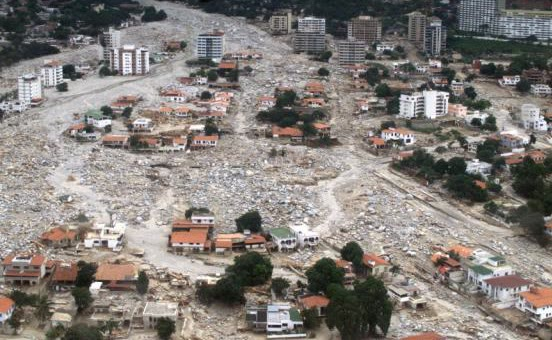
\includegraphics[width=0.62\linewidth]{images/book4/b2-28-caraballeda-debris-flow.jpg}
\par\smallskip{\small वेनेज़ुएला के तट पर कराबायेदा के पंखे पर \omterm{def:b2:geological-hazards:slope}{मलबा-प्रवाह} निक्षेप,
दिसंबर 1999 के तूफ़ान के बाद: प्रवाह मुख्य वाहिका से निकलकर नगर को गोलाश्मों के नीचे
दबा गए। फ़ोटो: Lawson Smith, U.S. Army Corps of Engineers (सार्वजनिक डोमेन)।}
\end{omfigure}
% ledger: photo:b2-28-caraballeda, vargas:caraballeda

\section{सुनामी}\label{sec:b2:geological-hazards:tsunamis}

समुद्र-तल के आकस्मिक उत्थान से उठी सुनामी की तरंगदैर्ध्य दसियों से सैकड़ों
किलोमीटर होती है, महासागर की गहराई से कहीं अधिक। वह एक दीर्घ तरंग है, और उसका वेग केवल
गहराई पर निर्भर करता है।

\begin{proposition}[दीर्घ तरंगें]\label{prop:b2:geological-hazards:long-waves}
जल की गहराई $h$ से बहुत बड़ी तरंगदैर्ध्य वाली एक सतही गुरुत्व तरंग, अपनी तरंगदैर्ध्य चाहे जो हो,
$c = \sqrt{gh}$ से चलती है। जहाँ वह परावर्तित हुए या टूटे बिना धीरे-धीरे उथले जल में जाती है,
वहाँ उसका आयाम $A$, $h^{-1/4}$ के रूप में बढ़ता है।
\end{proposition}

\begin{proof}
परिक्षेपण संबंध कला-वेग $c = \omega/k = \sqrt{(g/k)\tanh(kh)}$ देता है। एक दीर्घ
तरंग के लिए $kh = 2\pi h/\lambda \ll 1$, और $\tanh(kh) \approx kh$, अतः $c = \sqrt{gh}$, जो
$k$ से स्वतंत्र है: दीर्घ तरंगें परिक्षेपित नहीं होतीं। समुद्र-सतह के प्रति इकाई क्षेत्रफल तरंग की ऊर्जा $\frac12
\rho g A^2$ है, और वह $c$ से चलती है। यदि कोई ऊर्जा परावर्तित या नष्ट न हो, तो किसी भी अनुप्रस्थ काट से प्रवाह $\frac12\rho g A^2
c$ पथ के अनुदिश समान रहता है: $A^2 \sqrt{h}$ स्थिर है, और $A \propto
h^{-1/4}$।
\end{proof}

\qty{4000}{m} जल के ऊपर सुनामी \qty{198}{m.s^{-1}}, यानी \qty{713}{km/h}, से चलती है;
\qty{5000}{m} के ऊपर \qty{797}{km/h}, चेतावनी सेवाओं द्वारा उद्धृत ``800 km/h से अधिक''। तट के
निकट, \qty{10}{m} जल में, वह धीमी होकर \qty{36}{km/h} रह जाती है; पीछे का जल उसके अग्र भाग को पकड़ लेता है,
तरंग छोटी और खड़ी होती जाती है, और उसकी ऊँचाई बढ़ती है।
% ledger: nws:tsunami-speed

\begin{definition}[सुनामी आरोहण]\label{def:b2:geological-hazards:tsunami}
तट के किसी बिंदु पर \emph{सुनामी आरोहण}\index{सुनामी आरोहण} उस समय के समुद्र-तल से ऊपर, उस सबसे ऊँची
भूमि की ऊँचाई है जहाँ तक जल वहाँ अंतःस्थल में पहुँचता है। तटरेखा से उस बिंदु तक की क्षैतिज
दूरी जलप्लावन दूरी है।
\end{definition}

सर्वेक्षण दल हर सुनामी के बाद जल-चिह्नों, मलबा-रेखाओं और क्षति से आरोहण मापते हैं।
वैश्विक सुनामी डेटाबेस में 26 दिसंबर 2004 की हिंद महासागर सुनामी के लिए, जो सुमात्रा के तट से दूर
9.1 परिमाण के भूकंप से उठी थी, \num{2177} आरोहण प्रेक्षण हैं, जिनमें अधिकतम जल-ऊँचाई
\qty{50.9}{m} है, और होंशू के तट से दूर 11 मार्च 2011 की सुनामी के लिए, जो भी 9.1 परिमाण की थी, \num{6429},
जिनमें अधिकतम \qty{39.3}{m} है। दोनों ने \num{227899} और \num{18423} लोगों की जान ली। बांदा आचेह में
जल नीचे दिखाई गई मस्जिद की दूसरी मंज़िल के मध्य तक पहुँचा।
% ledger: ncei:tsu-2004, ncei:tsu-2011, usgs:aceh-mosque

\begin{omfigure}
\centering
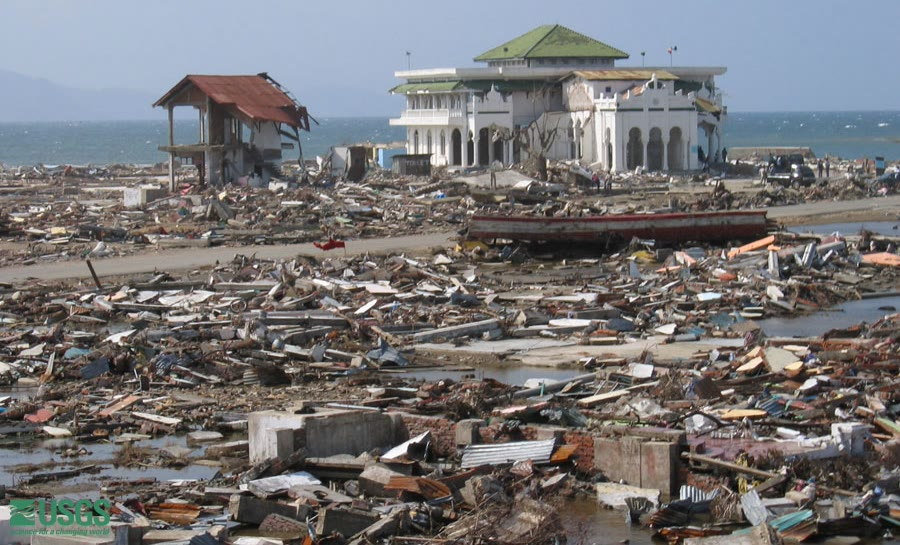
\includegraphics[width=0.62\linewidth]{images/book4/b2-28-aceh-mosque-tsunami.jpg}
\par\smallskip{\small बांदा आचेह, सुमात्रा, 21 जनवरी 2005 को, 26 दिसंबर 2004 की
सुनामी के बाद: आसपास के भवनों के मलबे के बीच एक मस्जिद खड़ी है। फ़ोटो: U.S. Geological
Survey (सार्वजनिक डोमेन)।}
\end{omfigure}
% ledger: photo:b2-28-aceh

\section{बाढ़}\label{sec:b2:geological-hazards:floods}

\begin{definition}[बाढ़ आवृत्ति वक्र]\label{def:b2:geological-hazards:flood}
किसी मापन स्टेशन पर किसी नदी का \emph{बाढ़ आवृत्ति वक्र}\index{बाढ़ आवृत्ति वक्र}
उसके \omterm{def:b2:geological-hazards:return}{पुनरावृत्ति काल}, या उसकी वार्षिक \omterm{def:b2:geological-hazards:poisson}{अतिक्रमण प्रायिकता}, के सापेक्ष वार्षिक शिखर विसर्जन का
वक्र है, जो स्टेशन के वार्षिक शिखरों के अभिलेख से बनाया जाता है और प्रायः एक समंजित
प्रायिकता नियम से बढ़ाया जाता है।
\end{definition}

स्कूल की पुस्तकों का कोटि-सूत्र वक्र के बिंदुओं को स्थापित करता है। उसका एक कारण है।

\begin{proposition}[वाइबुल आलेखन स्थिति]\label{prop:b2:geological-hazards:weibull}
मान लीजिए $n$ वार्षिक शिखर स्वतंत्र हैं और एक ही संतत बंटन से लिए गए हैं, और
$G(x)$ यह प्रायिकता है कि किसी वर्ष का शिखर $x$ से अधिक हो। सबसे बड़े से गिनी गई कोटि $m$ के
शिखर की अपेक्षित \omterm{def:b2:geological-hazards:poisson}{अतिक्रमण प्रायिकता} $m/(n + 1)$ है, जिससे उसे $T = (n +
1)/m$ पर आलेखित किया जाता है।
\end{proposition}

\begin{proof}
किसी संतत नियम के लिए $U = G(X)$, $[0, 1]$ पर एकसमान है, और $G$ ह्रासमान है, अतः
$m$-वाँ सबसे बड़ा शिखर $m$-वें सबसे छोटे के संगत है, $n$ स्वतंत्र एकसमान चरों में से,
$U_{(m)}$। उसका घनत्व $f(u) = \frac{n!}{(m-1)!\,(n-m)!}u^{m-1}(1-u)^{n-m}$ है: $n$ मानों में से एक
$u$ पर, $m - 1$ नीचे और $n - m$ ऊपर। बीटा समाकल $\int_0^1 u^{p}(1-u)^{q}\,\mathrm{d}u
= p!\,q!/(p + q + 1)!$ के साथ,
\begin{equation*}
\mathbb{E}[U_{(m)}] = \frac{n!}{(m-1)!\,(n-m)!}\cdot\frac{m!\,(n-m)!}{(n+1)!} = \frac{m}{n+1}. \qedhere
\end{equation*}
\end{proof}

इस प्रकार 30 वर्षीय अभिलेख का सबसे बड़ा शिखर 31 वर्ष पर आलेखित होता है, और अभिलेख में कुछ भी
100-वर्षीय बाढ़ को निश्चित नहीं करता। उस तक पहुँचने के लिए शिखरों पर एक चरम-मान नियम समंजित किया जाता है, प्रायः गंबेल का,
$\Pr(\text{शिखर} \leq x) = \exp\bigl(-e^{-(x - u)/\alpha}\bigr)$, जिसकी $T$-वर्षीय बाढ़ $x_T = u
- \alpha\ln\bigl(-\ln(1 - 1/T)\bigr)$ है: $-\ln(-\ln(1 - 1/T))$ के सापेक्ष एक सीधी रेखा, जिसे
अभिलेख से आगे उस जोखिम पर बहिर्वेशित किया जाता है जो दूरी के साथ बढ़ता है।

\section{निगरानी और पूर्व चेतावनी}\label{sec:b2:geological-hazards:warning}

\begin{definition}[पूर्व चेतावनी प्रणाली]\label{def:b2:geological-hazards:warning}
\emph{पूर्व चेतावनी प्रणाली}\index{पूर्व चेतावनी प्रणाली} संकट-निगरानी,
पूर्वानुमान, जोखिम-मूल्यांकन, संचार और तैयारी की एक एकीकृत प्रणाली है जो किसी
संकटपूर्ण घटना से पहले समय पर कार्रवाई संभव बनाती है। वह चार तत्वों को जोड़ती है: जोखिम का ज्ञान; संकट का संसूचन,
निगरानी और पूर्वानुमान; चेतावनियों का प्रसार; और अनुक्रिया की
तैयारी।
\end{definition}
% ledger: undrr:ews

भौतिकी तय करती है कि हर चेतावनी कितना समय दे सकती है। भूकंपीय तरंगों से आगे नहीं भागा जा सकता, पर हानिकारक
S तरंगें ऊपरी भूपर्पटी में लगभग \qty{3.2}{km.s^{-1}} से चलती हैं, जबकि
P तरंगें \qty{5.8}{km.s^{-1}} से: अधिकेंद्र के निकट अभिलिखित पहली P तरंगों से परिकलित एक चेतावनी किसी नगर तक
S तरंगों से पहले पहुँचती है, $d(1/3.2 - 1/5.8) = \qty{0.14}{s}$ पहले, दूरी $d$ के प्रति किलोमीटर, जिसमें से
संसूचन और परिकलन का समय घटाना होता है। \qty{100}{km} दूर का नगर अधिकतम \qty{14}{s} पाता है; स्रोत के निकट एक
अंध क्षेत्र कुछ नहीं पाता (\cref{exo:b2:geological-hazards:12})। \qty{100}{km}
पार करती सुनामी, \qty{2000}{m} गहरे समुद्र में, 12 मिनट लेती है; किसी महासागर के आर-पार वह घंटे लेती है। 2011 में जापानी
चेतावनी भूकंप के लगभग तीन मिनट बाद जारी हुई, पर बहुत कम आँके गए परिमाण पर,
क्योंकि उपकरण संतृप्त हो गए थे; उसे लगभग 28 मिनट बाद अपतटीय GPS प्लव के आँकड़ों से अद्यतन किया गया।
गहरे महासागर के दाब-अभिलेखक, जो हर 15 सेकंड में समुद्र-तल पर दाब को
समुद्र-सतह की ऊँचाई में बदलते हैं, अब गुज़रती सुनामियों की सूचना उपग्रह द्वारा देते हैं।
% ledger: data:prem, jma:warning, ndbc:dart
% values: 0.1401 s/km, 14.0 s at 100 km; 140 m/s over 2000 m, 11.9 min per 100 km (calc/ch28.py)

\begin{inthefield}[एक ढाल को खिसकते देखना]
किसी ऐसी ढाल पर जिसका सर्पण ज्ञात है, निगरानी दल ऐसे उपकरण लगाते हैं जो
अनंत-ढाल समीकरण के चरों को मापते हैं। वेधछिद्रों में पीज़ोमीटर सर्पण सतह पर छिद्र-दाब अभिलिखित करते हैं;
गहराई के अंतरालों पर पढ़ी जाने वाली नतिमापी नलिकाएँ दिखाती हैं कि भूमि कहाँ मुड़ती है और कितनी तेज़ी से; GNSS
स्टेशन और विस्तारमापी सतह की गति अभिलिखित करते हैं; एक वर्षामापी प्रेरक को अभिलिखित करता है।
दल गति की तुलना वर्षा और जल-दाब से करते हैं, ऋतु-दर-ऋतु, और विफलता से पहले आने वाले
त्वरण को खोजते हैं।
\end{inthefield}

\section*{अभ्यास}\label{sec:b2:geological-hazards:exercises}

अभ्यासों के आँकड़े, अन्यथा न कहा जाए तो: $g = \qty{9.81}{m.s^{-2}}$; जल का इकाई भार
\qty{9.81}{kN.m^{-3}}; चट्टान पर GMPE \eqref{eq:b2:geological-hazards:gmpe} ($G_B = G_C = 0$),
$\sigma = 0.230$; ऊपरी भूपर्पटी में P और S वेग 5.8 और \qty{3.2}{km.s^{-1}}। तीन
सार्थक अंकों तक पूर्णांकित कीजिए।
% ledger: bjf93:pga, data:prem

\begin{exercise}[$\star$]\label{exo:b2:geological-hazards:1}
प्वासों मॉडल के अंतर्गत: (क)~30 वर्षों में कम से कम एक 100-वर्षीय बाढ़ की प्रायिकता क्या है?
(ख)~इसकी प्रायिकता क्या है कि एक शताब्दी 100-वर्षीय बाढ़ के बिना बीत जाए? (ग)~50 वर्षों में
\qty{5}{\percent} अतिक्रमण-संभावना वाली गति का \omterm{def:b2:geological-hazards:return}{पुनरावृत्ति काल} ज्ञात कीजिए।
\end{exercise}

\begin{exercise}[$\star$]\label{exo:b2:geological-hazards:2}
दो कस्बे प्रबल कंपन का सामना करते हैं। कस्बे A में वह 200 वर्षों में एक बार की दर से होता है और
उसके 5000 भवनों में से \qty{2}{\percent} नष्ट कर देगा; कस्बे B में 50 वर्षों में एक बार, उसके 800 भवनों में से
\qty{10}{\percent} नष्ट करते हुए। (क)~हर कस्बे में प्रति वर्ष नष्ट होने वाले भवनों की अपेक्षित संख्या
ज्ञात कीजिए। (ख)~किस कस्बे का जोखिम अधिक है, यद्यपि उसका \omterm{def:b2:geological-hazards:risk}{उद्भासन} कम है? (ग)~तीन
गुणकों में से कौन-सा अंतर पैदा करता है?
\end{exercise}

\begin{exercise}[$\star$]\label{exo:b2:geological-hazards:3}
(क)~4000, 200 और \qty{10}{m} की गहराइयों पर सुनामी का वेग ज्ञात कीजिए। (ख)~\qty{1500}{km}
महासागर, \qty{4000}{m} गहरा, पार करने में उसे कितना समय लगता है? (ग)~किस गहराई पर वह
\qty{800}{km/h} से चलेगी?
\end{exercise}

\begin{exercise}[$\star$]\label{exo:b2:geological-hazards:4}
$\varphi' = \ang{33}$ वाली एक शुष्क, संसंजनहीन रेत एक लंबी ढाल बनाती है। (क)~\ang{25} पर उसका \omterm{def:b2:geological-hazards:slope}{सुरक्षा
गुणक} ज्ञात कीजिए। (ख)~वह सबसे खड़ी ढाल कौन-सी है जो वह बना सकती है? (ग)~ढाल संतृप्त हो जाती है,
जलस्तर सतह पर और रिसाव उसके समांतर, जिससे $r_u = \gamma_w\cos^2\beta/\gamma$,
जहाँ $\gamma = \qty{20}{kN.m^{-3}}$। दिखाइए कि $F = (1 - \gamma_w/\gamma)\tan\varphi'/\tan\beta$ और
\ang{25} पर उसका मान निकालिए।
\end{exercise}

\begin{exercise}[$\star\star$]\label{exo:b2:geological-hazards:5}
वैश्विक सूची में 1976--2025 के 50 वर्षों में कम से कम 7 परिमाण के 696 भूकंप हैं, और
उनके बीच का माध्य अंतराल 26.2 दिन है। (क)~उनकी माध्य वार्षिक दर ज्ञात कीजिए। (ख)~प्वासों
मॉडल के अंतर्गत, इसकी प्रायिकता क्या है कि 30 दिन बिना किसी के बीत जाएँ? 30 दिनों से लंबे अंतरालों के प्रेक्षित
अंश, 0.304, से तुलना कीजिए। (ग)~किसी दिए गए सप्ताह में कम से कम एक की
प्रायिकता क्या है?
\end{exercise}

\begin{exercise}[$\star\star$]\label{exo:b2:geological-hazards:6}
(क)~चट्टान पर 6.5 परिमाण के भूकंप का माध्यिका PGA $d = 0$, 10, 30 और
\qty{100}{km} पर ज्ञात कीजिए। (ख)~वर्ग C के स्थल पर \qty{10}{km} पर वह क्या होता? (ग)~चट्टान पर \qty{10}{km} पर
PGA लगभग \qty{68}{\percent} प्रायिकता के साथ किन मानों के बीच रहता है?
\end{exercise}

\begin{exercise}[$\star\star$]\label{exo:b2:geological-hazards:7}
12 वर्षों में किसी नदी के वार्षिक शिखर, \unit{m^3.s^{-1}} में, ये थे: 212, 148, 305, 176, 251, 133, 188,
420, 160, 229, 195, 268। (क)~चार सबसे बड़ों के \omterm{def:b2:geological-hazards:return}{पुनरावृत्ति काल} बताइए। (ख)~दो सबसे बड़ों के बीच
$\ln T$ में रैखिक अंतर्वेशन द्वारा 10-वर्षीय बाढ़ का आकलन कीजिए। (ग)~यह अभिलेख 100-वर्षीय बाढ़ के बारे में
कुछ भी विश्वसनीय क्यों नहीं बता सकता?
\end{exercise}

\begin{exercise}[$\star\star$]\label{exo:b2:geological-hazards:8}
एक अशांत ज्वालामुखी पर वेधशाला ये आकलन करती है: अशांति मैग्मीय 0.6; मैग्मीय होने पर उद्गार 0.4;
उद्गार होने पर विस्फोटी 0.5; विस्फोटी होने पर किसी दी गई घाटी तक पहुँचने वाला \omterm{def:b2:eruptive-styles:pdc}{पायरोक्लास्टिक प्रवाह} 0.3। (क)~घाटी में
\omterm{def:b2:eruptive-styles:pdc}{पायरोक्लास्टिक प्रवाह} की प्रायिकता ज्ञात कीजिए। (ख)~उद्गार की प्रायिकता ज्ञात कीजिए, और
घाटी में प्रवाह के बिना उद्गार की। (ग)~नए विरूपण-आँकड़े, अशांति के मैग्मीय होने पर, उद्गार की प्रायिकता को
0.7 तक बढ़ा देते हैं। (क) को अद्यतन कीजिए।
\end{exercise}

\begin{exercise}[$\star\star$]\label{exo:b2:geological-hazards:9}
$c' = \qty{8}{kPa}$, $\varphi' = \ang{30}$ और $\gamma = \qty{19}{kN.m^{-3}}$ वाली एक शुष्क मृदा
\ang{35} की ढाल पर टिकी है। (क)~वह मोटाई $z_c$ ज्ञात कीजिए जिस पर $F = 1$। (ख)~$F$ ज्ञात कीजिए,
एक \qty{2}{m} मोटी परत के लिए। (ग)~वही परत संतृप्त हो जाती है, जलस्तर सतह पर और
$r_u = \gamma_w\cos^2\beta/\gamma$। $F$ ज्ञात कीजिए।
\end{exercise}

\begin{exercise}[$\star\star\star$]\label{exo:b2:geological-hazards:10}
(क)~दिखाइए कि प्वासों मॉडल स्मृतिहीन है: $[s, s + t]$ में कोई घटना न होने की प्रायिकता,
यह दिया होने पर कि $[0, s]$ में कोई नहीं हुई, $e^{-t/T}$ है, $s$ चाहे जो हो। (ख)~किसी भ्रंश के बड़े भूकंपों का
\omterm{def:b2:geological-hazards:return}{पुनरावृत्ति काल} 475 वर्ष है और 400 वर्षों से कोई नहीं हुआ। मॉडल के अंतर्गत अगले 50 वर्षों में
एक की प्रायिकता क्या है? (ग)~पुस्तक 3 (स्नातक वर्ष 1) का प्रत्यास्थ प्रतिक्षेप सुझाता है कि प्रायिकता को
इसके बजाय पिछले भूकंप के बाद के समय के साथ बढ़ना चाहिए। यह प्वासों मॉडल की किस मान्यता का खंडन करता है,
और संकट मानचित्र क्षेत्रीय स्रोतों के लिए मॉडल को क्यों बनाए रखते हैं?
\end{exercise}

\begin{exercise}[$\star\star\star$]\label{exo:b2:geological-hazards:11}
\qty{0.5}{m} आयाम और 20 मिनट आवर्तकाल की एक सुनामी \qty{4000}{m} गहरे महासागर को पार करती है। (क)~दीर्घ
तरंगों वाली प्रतिज्ञप्ति के ऊर्जा-प्रवाह तर्क का उपयोग करके \qty{10}{m} जल में उसका आयाम
ज्ञात कीजिए। (ख)~दोनों गहराइयों पर उसकी तरंगदैर्ध्य ज्ञात कीजिए। (ग)~दो कारण बताइए कि तट पर आरोहण
इस आकलन से बहुत भिन्न क्यों हो सकता है।
\end{exercise}

\begin{exercise}[$\star\star\star$]\label{exo:b2:geological-hazards:12}
एक भूकंप \omterm{def:b2:geological-hazards:warning}{पूर्व चेतावनी प्रणाली} अधिकेंद्र से निकटतम अपने स्टेशन तक, जो \qty{10}{km} दूर है, P तरंग पहुँचने के
4 सेकंड बाद चेतावनी जारी करती है। स्रोत की गहराई की उपेक्षा कीजिए। (क)~भूकंप के कितने समय बाद
चेतावनी जारी होती है? (ख)~अधिकेंद्र से \qty{50}{km} दूर का कस्बा उसे S तरंग से कितने सेकंड पहले
पाता है? \qty{100}{km} पर का कस्बा? (ग)~अंध क्षेत्र की त्रिज्या ज्ञात कीजिए, जहाँ
S तरंग चेतावनी से पहले पहुँचती है।
\end{exercise}

\begin{problem}[{सप्ताहांत समस्या --- एक भ्रंश और एक ढाल के बीच एक कस्बा}]\label{pb:b2:geological-hazards:1}
चट्टान पर बसा एक कस्बा किसी स्रोत क्षेत्र से \qty{10}{km} दूर है; उसके सभी भूकंप
$d = \qty{10}{km}$ पर लिए जाते हैं। उनकी पुनरावृत्ति प्रति वर्ष $\log_{10} N(\geq M) = 4.0 - 1.0\,M$ है, $M \geq 5$ के लिए,
$M_{\max} = 7.5$ पर छाँटी गई। कंपन $\sigma = 0.230$ के साथ GMPE \eqref{eq:b2:geological-hazards:gmpe}
का अनुसरण करता है। कस्बे के ऊपर, \qty{3}{m} मोटी मृदा की एक परत \ang{30} की ढाल पर टिकी है,
जहाँ $\gamma = \qty{19}{kN.m^{-3}}$, $c' = \qty{4}{kPa}$ और $\varphi' = \ang{34}$; जल का इकाई
भार \qty{9.81}{kN.m^{-3}} है। तीन सार्थक अंकों तक पूर्णांकित कीजिए।

\noindent\textbf{भाग I --- पुनरावृत्ति।}
\begin{enumerate}
  \item छँटाई की उपेक्षा करते हुए, कम से कम 5, 6 और 7 परिमाण के भूकंपों की वार्षिक दरें
        ज्ञात कीजिए।
  \item संगत \omterm{def:b2:geological-hazards:return}{पुनरावृत्ति काल} बताइए।
  \item छँटाई के साथ, 7.5 से ऊपर के भूकंपों की दर, और 7
        और 7.5 के बीच वालों की दर ज्ञात कीजिए।
  \item परिमाण-खानों 5--6 और 6--7 की दरें ज्ञात कीजिए।
  \item 50 वर्षों में 6 या अधिक परिमाण के कम से कम एक भूकंप की प्रायिकता क्या है?
  \item और 7 या अधिक परिमाण के?
\end{enumerate}

\noindent\textbf{भाग II --- कस्बे पर भू-गति।}
\begin{enumerate}[resume]
  \item $r$, और दूरी-पद $-0.778\log_{10} r$ ज्ञात कीजिए।
  \item तीनों खानों को परिमाणों 5.5, 6.5 और 7.25 से निरूपित कीजिए। हर एक का माध्यिका
        $\log_{10}\mathrm{PGA}$ और माध्यिका PGA ज्ञात कीजिए।
  \item 6.5 परिमाण द्वारा \qty{16}{\percent} प्रायिकता के साथ अतिक्रमित PGA ज्ञात कीजिए।
  \item इसकी प्रायिकता क्या है कि 6.5 परिमाण \qty{0.3}{g} से अधिक उत्पन्न करे?
  \item सबसे बड़े संभव भूकंप का माध्यिका PGA क्या है?
\end{enumerate}

\noindent\textbf{भाग III --- संकट वक्र।}
\begin{enumerate}[resume]
  \item तीनों खानों पर योग करके, \qty{0.2}{g} के अतिक्रमण की वार्षिक दर ज्ञात कीजिए।
  \item \qty{0.3}{g} के लिए वही।
  \item \qty{0.4}{g} के लिए वही।
  \item 50 वर्षों में \qty{10}{\percent} के संगत वार्षिक दर क्या है?
  \item वह दर तीनों स्तरों में से किन दो के बीच पड़ती है?
  \item $\ln\lambda$ में, $\ln a$ के सापेक्ष, रैखिक अंतर्वेशन करके, 50 वर्षों में
        \qty{10}{\percent} अतिक्रमण-संभावना वाला PGA ज्ञात कीजिए।
  \item \qty{0.3}{g} पर दर में कौन-से खाने सबसे अधिक योगदान देते हैं? प्रश्न~11 के उत्तर का उपयोग करते हुए
        टिप्पणी कीजिए।
\end{enumerate}

\noindent\textbf{भाग IV --- कस्बे के ऊपर की ढाल।}
\begin{enumerate}[resume]
  \item शुष्क ढाल का \omterm{def:b2:geological-hazards:slope}{सुरक्षा गुणक} ज्ञात कीजिए।
  \item जब परत संतृप्त हो, जलस्तर सतह पर ($r_u =
        \gamma_w\cos^2\beta/\gamma$), तब उसे ज्ञात कीजिए।
  \item ढाल के विफल होने से पहले जलस्तर परत की मोटाई के किस अंश तक उठ सकता है?
  \item एक छद्म-स्थैतिक विश्लेषण (स्वीकृत) में कंपन एक क्षैतिज बल $kW$ जोड़ता है। शुष्क ढाल का
        क्रांतिक $k$ ज्ञात कीजिए, जिस पर $F = 1$।
  \item $k$ को $g$ की इकाइयों में PGA के बराबर लेते हुए, कौन-सा परिमाण कस्बे पर अपनी माध्यिका के रूप में
        क्रांतिक मान उत्पन्न करता है? प्रश्न~17 के उत्तर से तुलना कीजिए।
  \item सारांश में: कस्बे पर 50 वर्षों में अतिक्रमित होने की \qty{10}{\percent} संभावना वाला
        \omterm{def:b2:geological-hazards:psha}{शिखर भू-त्वरण} क्या है?
\end{enumerate}
\end{problem}
